\chapter{\ttZ\ estimation for a Dark Matter search}
\markboth{}{Appendix A}
\label{app:ttzdm}

	The data-driven background estimation technique, already discussed in Section~\ref{sec:ddbkgest}, and the theory uncertainties calculation prescription presented in Section~\ref{sec:syst_unc}, were also used in the search for dark matter produced in association with third-generation quarks, which was published in October $2017$ in the \EPJ~\cite{DMhf}. The author's contribution to this analysis only regarded the \ttZ\ background estimation and the computation of the relevant theory uncertainties and, as such, only these two topics will be hereby covered.


	\section{Overview of the analysis}

		\begin{table}[!htb]
			\caption{Summary of the kinematic and topology-dependent selections for signal regions SRt1 and SRt2~\cite{DMhf}. SRt3 is not reported as it was not relevant for the estimation of the \ttZ\ background.}
			\centering
			\renewcommand{\arraystretch}{1.5}
				\begin{tabular}{lcc}
					\toprule
					\textbf{Observable}  & SRt1 & SRt2 \\
					\midrule
					Trigger             &   \multicolumn{2}{c}{\met}   \\
					\antikt\ $R=0.4$ jets  & \multicolumn{2}{c}{$\ge 4,~\pt>80,80,40,40 \gev$} \\
					$N_{\bjs}$  & \multicolumn{2}{c}{$\geq2$} \\[0.3ex]
					$N_{\ell}$  & \multicolumn{2}{c}{$0$} \\[0.3ex]
					\midrule
					\met\ [\GeV]         &\multicolumn{2}{c}{$>300$}  \\
					$\pt$ leading \bj\ [\GeV] &  \multicolumn{2}{c}{$>20$}   \\
					\midrule
					\mantikteightzero\ [\GeV] & $>80$ & -     \\
					\mantikteightone\ [\GeV] & $>80$ & -     \\
					\mtbmin\ [\GeV]           & $>150$ & $>200$ \\
					\mtbmax\ [\GeV]           & $>250$ & -      \\
					\drbb\    & \multicolumn{2}{c}{$>1.5$} \\
					\metsig\  [$\sqrt{\GeV}$] & - & $>12$ \\
					\midrule
					%\multicolumn{3}{l}{Multi-jet rejection specific} \\
					\dphimin\ [rad]     &  \multicolumn{2}{c}{$>0.4$} \\
					\mettrack [\GeV]   &  \multicolumn{2}{c}{$> 30$}  \\
					$\Delta\phi(\ptmiss,\ptmisstrk)$  [rad] & \multicolumn{2}{c}{$< \pi/3$} \\
					\bottomrule
				\end{tabular}
			\label{tab:srtselections}
		\end{table}

		\begin{wrapfigure}{R}{.33\textwidth}
			\centering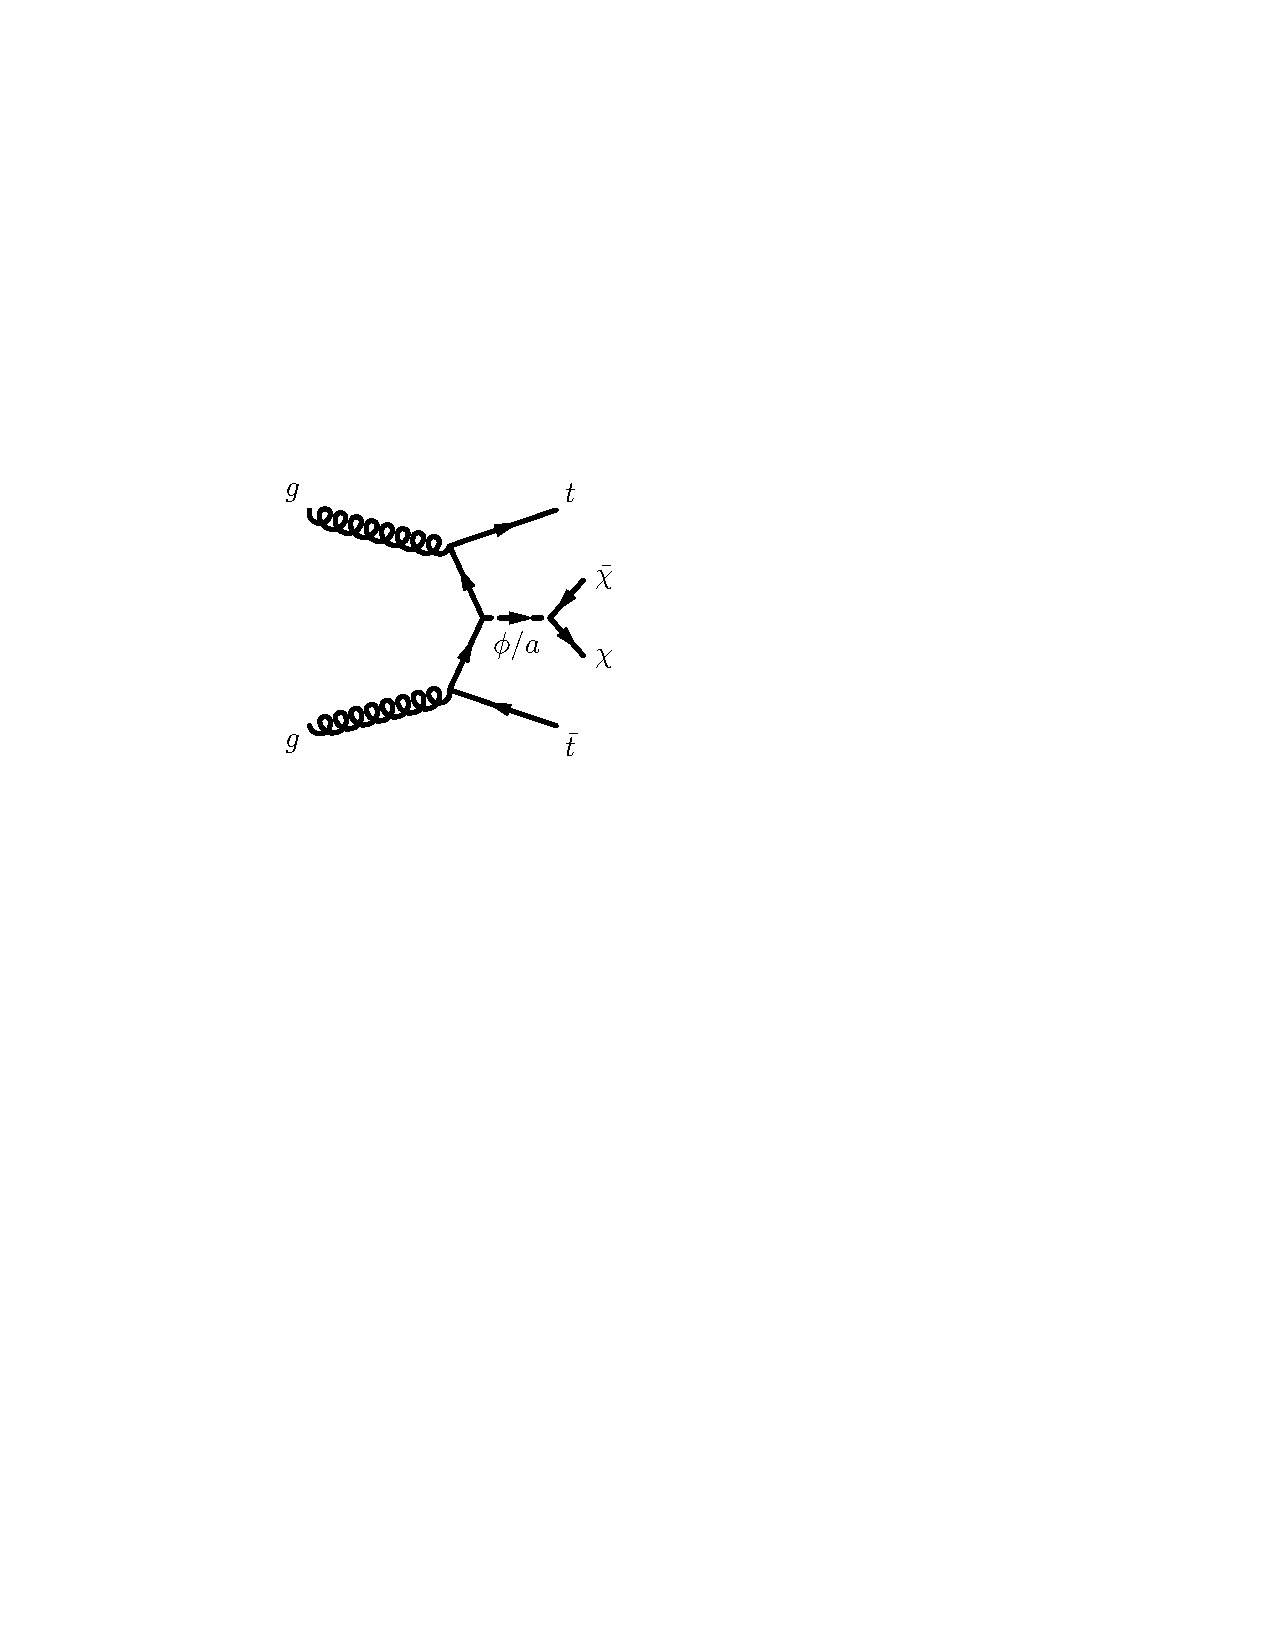
\includegraphics[width=.3\textwidth]{appA/TTphi}
			\caption{Representative diagram at the lowest order for spin-0 mediator associated production with top quarks $\ttbar+\phi/a$ (taken from~\cite{DMhf}).}
			\label{fig:dmhfModels}
		\end{wrapfigure}

		The analysis also used $36.1\, \ifb$ of \pp\ collisions delivered by the \ac{LHC} and recorded with the \ac{ATLAS} detector, and it targeted final states with either bottom- or top-quark pairs and missing transverse momentum. In particular, only the final state with two top quarks and missing transverse momentum, as shown in Figure~\ref{fig:dmhfModels}, will be considered here. The $0\ell$ final state of this analysis essentially yields an experimental signature identical to the one discussed in Chapter~\ref{ch:stop_ana}, namely 4 or more jets, two of which $b$-tagged, and missing transverse momentum. For such reason, the physics objects used in this analysis, and the variables employed for the design of a \ttgamma\ \ac{CR} to estimate the \ttZ\ background, are the same as those already extensively discussed in Chapters~\ref{ch:stop_ana}, and~\ref{ch:bkgest}. 

		Five \acp{SR} are employed in this analysis: SRb1, SRb2, SRt1, SRt2, and SRt3. SRb1 and SRb2 are optimised for models in which \ac{DM} is produced in association with one or two $b$-quarks and these will not be further considered as the author did not contribute to this part of the analysis. SRt1, SRt2, and SRt3, are optimised to isolate events in which \ac{DM} is produced in association with a top-antitop pair, that either decays fully hadronically (SRt1 and SRt2) or dileptonically (SRt3)~\cite{DMhf}. While the $\ttZ(\to \nu\nu)$ is an irreducible background in SRt1 and SRt2, it is negligible in SRt3 and therefore such \ac{SR} will be neglected here. SRt1 and SRt2 have a very similar background composition as the one discussed in Chapter~\ref{ch:stop_ana} and they target low ($< 100$ \GeV) and high (between $100$ and $350$ \GeV) mediator mass assumptions, respectively. 
		%The two \acp{SR} have selections criteria which overlap. 
		%As the \ac{SR} optimisation strategy of this analysis did not affect the \ttZ\ background estimation, the design of such \acp{SR} will not be further discussed, although the \acp{SR}, where 
		Table~\ref{tab:srtselections} shows the SRt1 and SRt2 selections.% where the \ttZ\ background estimation was employed. 


	\section{The estimation of the irreducible \ttZ\ background}

		\begin{table}[!htb]
			\parbox{.45\linewidth}{
			\centering
			\captionof{table}{Summary of the CR$\gamma$ selection for the \ttZ\ background estimation.}\label{tab:CRcuts}
		   	\begin{tabular}{lc}
					\toprule
					\textbf{Observable} & CR$\gamma$ \\
					\midrule
					Trigger & photon\\
					$N_{\mathrm{jets}}$ & $\geq 4$ \\ 
					$N_{\bjs}$ & $\geq 2$ \\ \midrule
					$N_\gamma$ & $1$ \\ 
					$\pt^{\gamma}$ [\GeV] & $>150$ \\
					$N_\ell$ & $1$ \\ 
					$\pt(\ell_1)$ [\GeV] & $>28$ \\ \bottomrule
			  \end{tabular}
			}
			\hfill
			\parbox{.45\linewidth}{
			\centering
			\captionof{table}{Background composition of \ttgamma\ CR. Pre-fit yields, statistical and detector systematic uncertainties shown.}
			\label{tab:CRgamma_yields}
				\begin{tabular}{lc}
					\toprule
					\textbf{Process} & \textbf{Yield} \\
					\toprule
					\ttgamma & $89.50 \pm 2.02$ \\
					$V+\gamma$ & $5.01 \pm 1.12$ \\
					$\ttbar$ & $4.26 \pm 0.94$ \\
					$\ttV$ & $1.79 \pm 0.23$ \\
					single Top & $1.86 \pm 0.52$ \\
					$Z$ & $0.56 \pm 0.13$ \\
					$W$ & $0.03 \pm 0.01$ \\
					\midrule
					Total MC & $103.01 \pm 2.69$ \\
					Data & $124$ \\
					\midrule
					\multicolumn{2}{c}{\textbf{CR}{\bm{$\gamma$} purity} ( $87\%$)} \\ 
					\midrule
					$\mu_{\ttgamma}$ & $1.22 \pm 0.13$ \\
					\bottomrule
				\end{tabular}
			}
		\end{table}

		As in the $\tilde{t}0\ell$ analysis - the search for top squarks in all-hadronic final states presented in Chapters~\ref{ch:stop_ana},~\ref{ch:bkgest}, and~\ref{ch:results} - the \ttV\ events, and in particular \ttZ\ events where the $Z$ boson decays into neutrinos, represent an irreducible background for the \acp{SR} targeting dark matter produced in association with top quarks (Figure~\ref{fig:dmhfModels}). Once again, a data-driven approach is employed to estimate such background. In particular, events with $\pt^{\gamma} > m_{\mathrm Z}$ resembling $\ttZ(\nu\nu)$ ones are selected. The CR${\gamma}$ selection, detailed in Table~\ref{tab:CRcuts}, allows to select events with exactly one energetic tight photon and at least one lepton from the decay of the \ttbar\ system. Such \ac{CR} essentially is identical to the one in Table~\ref{tab:CRTTGamma} already shown in Section~\ref{sec:ddbkgest} (page \pageref{sec:ddbkgest}), except for the applied trigger which is a single-photon instead of a $1$-lepton trigger. This strategy was found to allow the \ac{CR} CR$\gamma$ to better mimic the hard kinematic requirements of the two \acp{SR} targeting the signal in Figure~\ref{fig:dmhfModels}~\cite{DMhf}. Finally, in order to mimic the expected missing transverse momentum spectrum of $Z\rightarrow\nu\bar{\nu}$ events, the \pt\ of the photon ($\pt^{\gamma}$) is vectorially added to the \ptmiss, to form a variable called \metprimeg.



	\section{Results}

		A normalisation factor for the \ttZ\ \ac{SM} background, $\mu_{\ttZ} = 1.22$, was obtained by performing the background-only fit - employing the same procedure discussed in Chapter~\ref{ch:results} - including all the \ac{SM} backgrounds. Figure~\ref{fig:metprimecrgamma} shows the distribution of \metprimeg\ in CR$\gamma$ where a very good data/MC agreement was found. Lastly, by employing the same procedure discussed in Section~\ref{sec:syst_unc} the theory uncertainties were computed and found to be between $6\%-10\%$ across the various \acp{SR}. Additionally, Table~\ref{tab:CRgamma_yields} shows the background composition of CR$\gamma$, where an $87\%$ purity was reached.

		\begin{figure}[!htb]
		\centering
			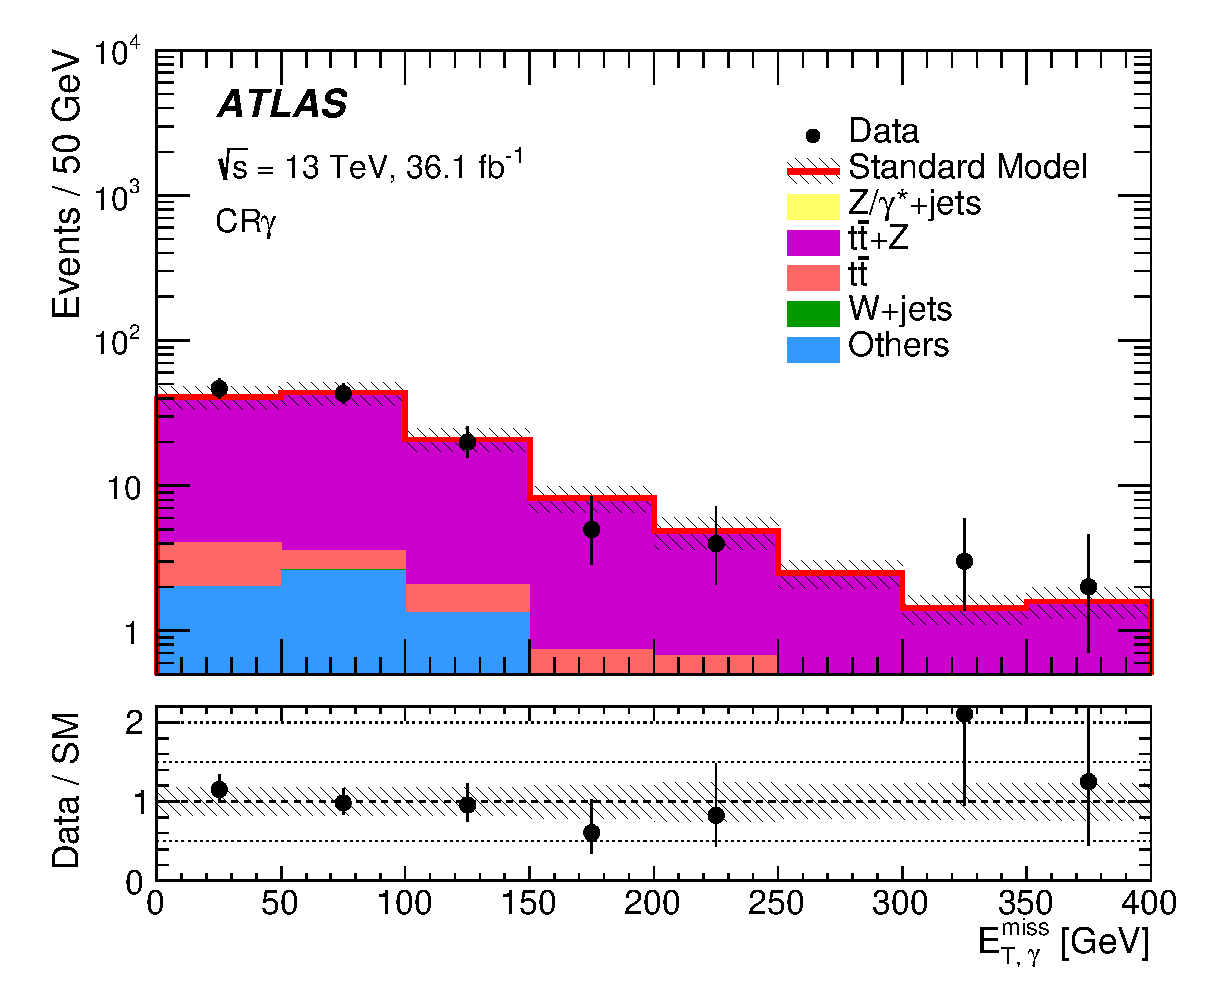
\includegraphics[width=.8\textwidth]{appA/can_CRttG_MetTST_met_afterFit}
			\caption{Comparison of the data with the post-fit Monte Carlo prediction of the \metprimeg\ distribution in CR$\gamma$. The bottom panel shows the ratio of the data to the \ac{MC} prediction. The band includes all systematic
			detector-related and theory uncertainties. The last bins include overflows, where applicable (taken from~\cite{DMhf}).}
			\label{fig:metprimecrgamma}
		\end{figure}

		The data is found to be compatible with the background prediction in each one of the \acp{SR}. In particular, in each \ac{SR} the observed yield in data is above the expected background but within $1.3$ standard deviations of its uncertainty, too low to suggest the presence of any of the searched signal. A model-independent fit~\cite{histfitter}, where both \acp{CR} and \acp{SR} are included, is employed to derive $95\%$ \ac{CL} upper limits on the visible cross-section of new \ac{BSM} processes, defined as cross-section times acceptance times efficiency ($\langle\sigma A \epsilon\rangle_{\mathrm obs}^{95}$) and obtained as the upper limit on the number of BSM events divided by the total integrated luminosity. No systematic uncertainties for the signal are assumed for such limits and any possible signal contamination in the \acp{CR} is neglected. %The results are also used to set limits on the production cross-section of colour-neutral and colour-charged mediator models decaying into dark-matter particles. When deriving model-dependent limits, the expected signal yield in each fit region is considered. 

		Figures~\ref{fig:dmresults} and~\ref{fig:dmresultschi} show upper limits at 95\% CL on $\sigma / \sigma (g = 1.0)$, namely the signal cross-section scaled to the signal cross-section for coupling $g = 1$. To derive the results for the fully hadronic \ttbar\ final state the region SRt1 or SRt2 with the best expected sensitivity is used. The SRt1 was originally optimised for low-mass scalar mediators, while SRt2 was optimised for high-mass scalar mediators and pseudoscalar mediators. However, SRt1 is strongly affected by systematic uncertainties in the \ttbar\ modelling and therefore SRt2 sets more stringent limits for the whole parameter space. These limits are obtained both as a function of the mediator mass, assuming a specific \ac{DM} mass of $1$ \GeV\ (Figure~\ref{fig:dmresults}), and as a function of the \ac{DM} mass, assuming a specific mediator mass of $10$ \GeV\ (Figure~\ref{fig:dmresultschi}). Both the scalar and pseudoscalar mediator cases are considered. The sensitivity for $\ttbar + \phi/a$ on-shell decays is approximately constant for masses below $100$ \GeV, with SRt3 excluding the $g = 1$ assumption for scalar mediator masses up to $50$ \GeV. For a given mediator mass the acceptance of the analysis is independent of the value of the \ac{DM} mass as long as $m(\phi / a) > 2  m(\chi)$ is fulfilled. Under these conditions, exclusion limits for \ac{DM} masses differing from the one presented can be inferred from the result shown in Figure~\ref{fig:dmresults}. Due to the smaller Yukawa enhancement of $\bbbar + \phi / a$ final states, it is possible to exclude cross-sections $300$ times the nominal values for $g = 1$.


		\begin{figure}[!htb]
			\centering
			\subbottom[]{
				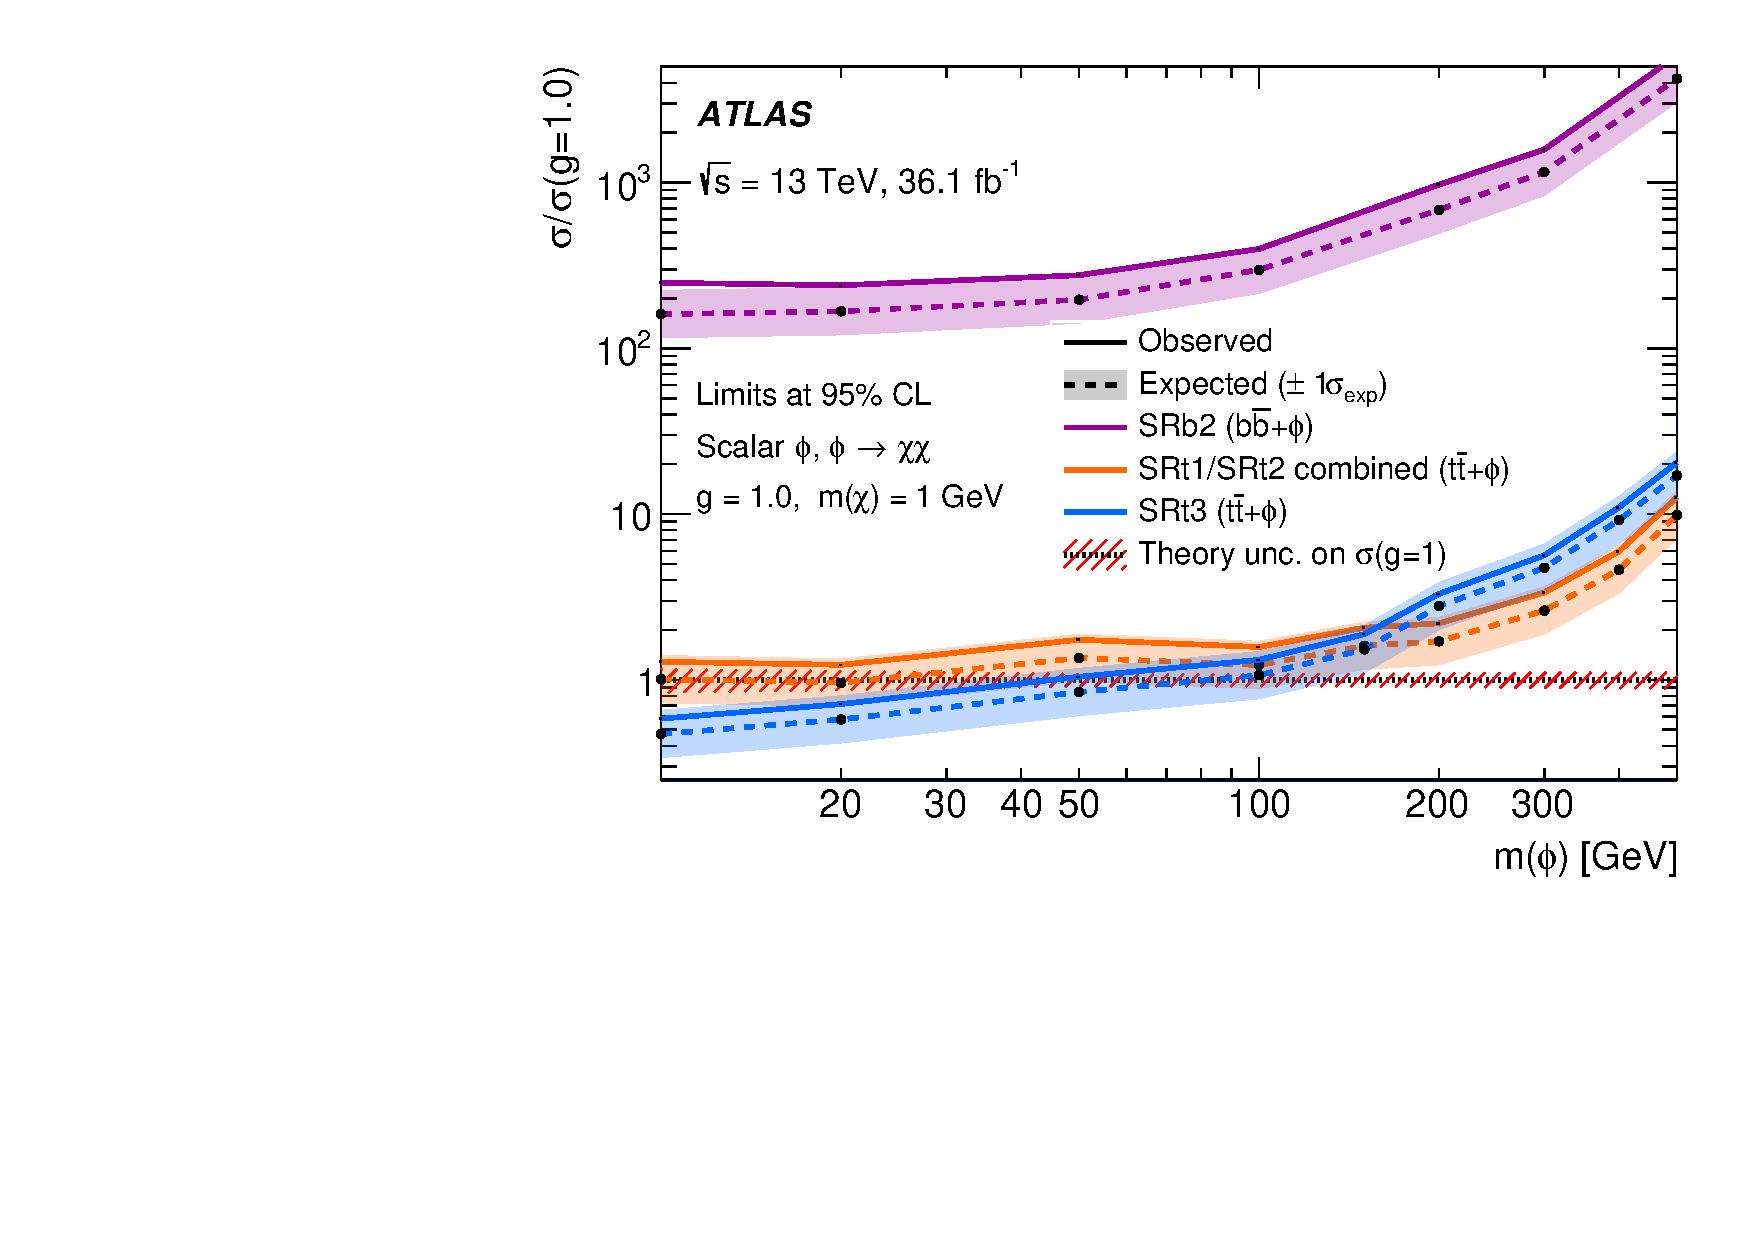
\includegraphics[width=.9\textwidth]{appA/final_scalar_SR1}}\\
			\subbottom[]{
				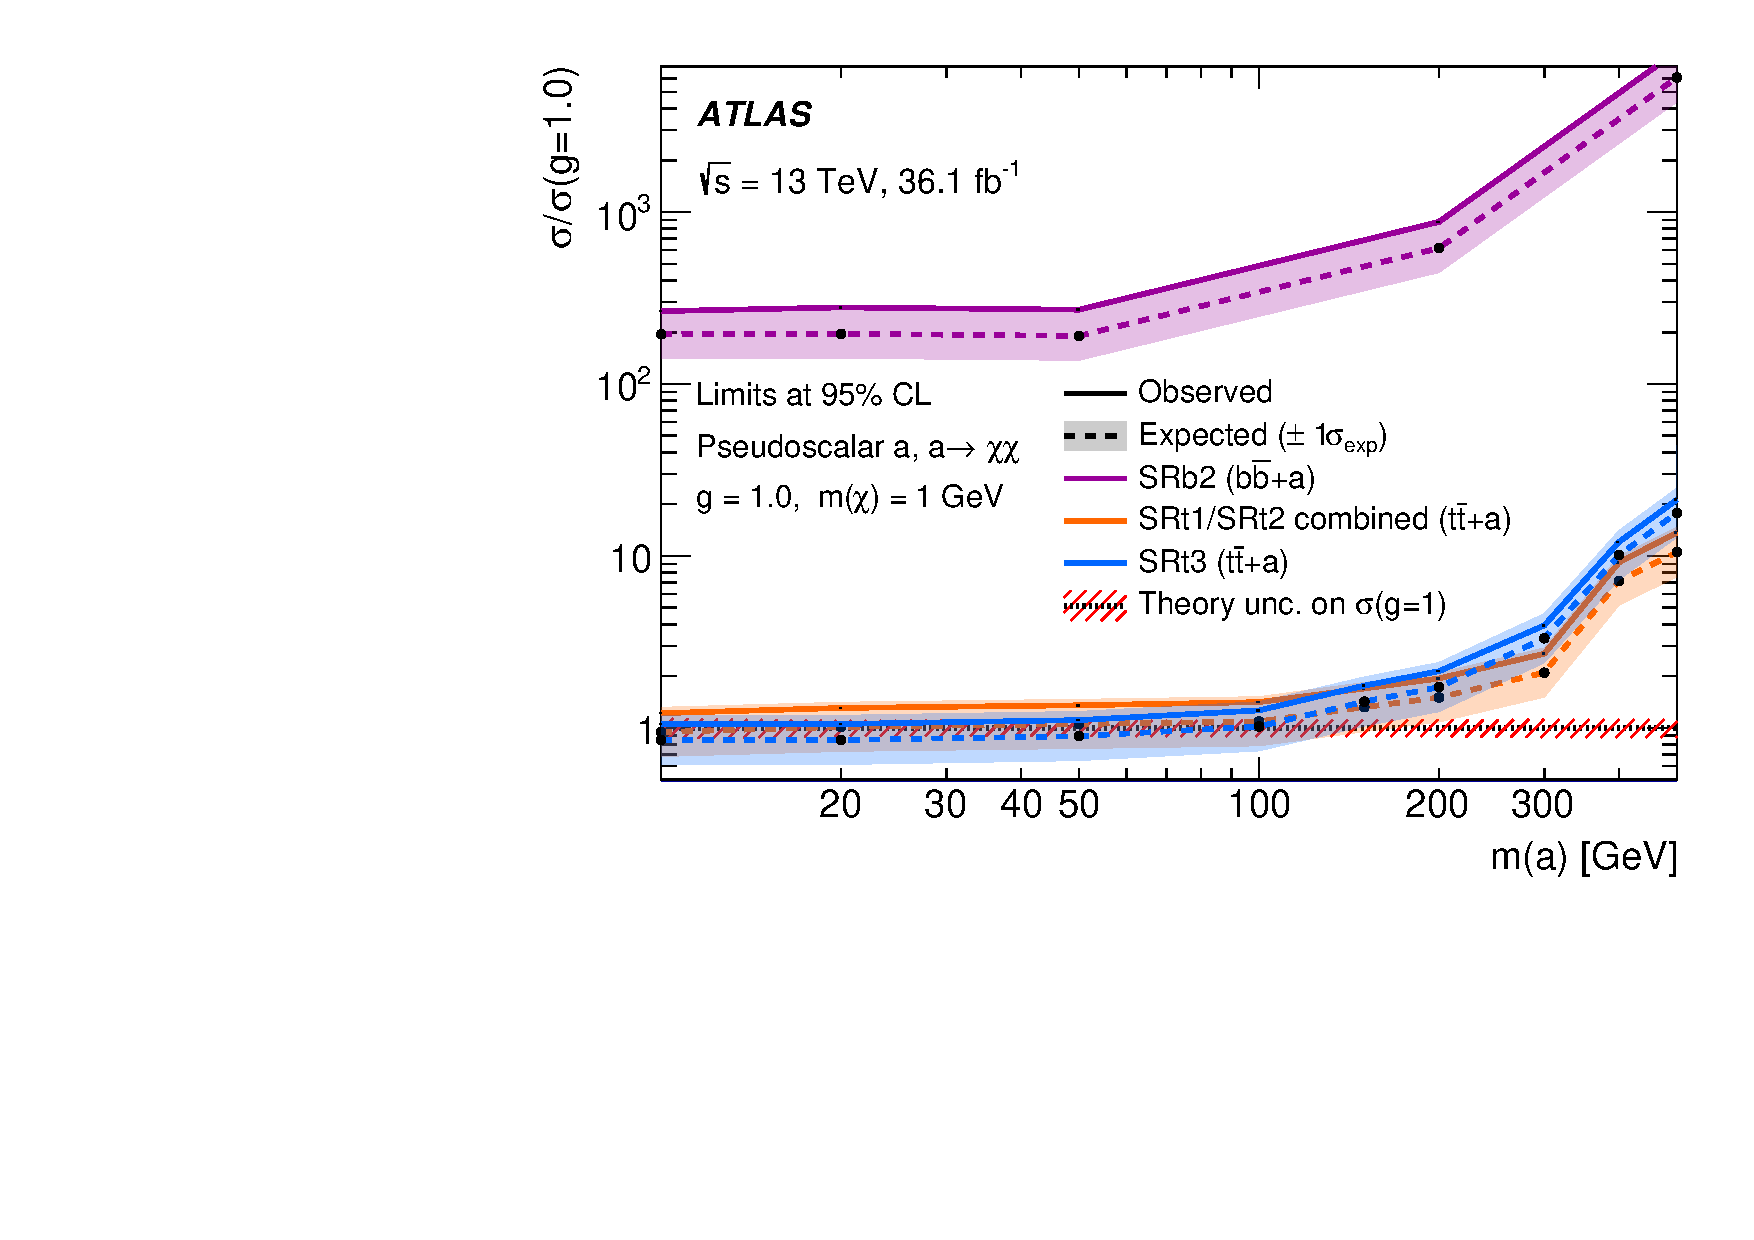
\includegraphics[width=.9\textwidth]{appA/final_pseudo_SR1}}
			\caption{Exclusion limits for colour-neutral $\ttbar/\bbbar+\phi$ scalar (a) and $\ttbar/\bbbar+a$ pseudoscalar (b) models as a function of the mediator mass for a DM mass of $1\;\GeV$. The limits are calculated at 95\% CL and are expressed in terms of the ratio of the excluded cross-section to the nominal cross-section for a coupling assumption of $g = g_q = g_\chi = 1$, where $g_\chi$ is the DM–mediator coupling, and $g_q$ the flavour-universal SM–mediator coupling. The solid (dashed) lines shows the observed (expected) exclusion limits for the different signal regions, according to the colour code specified in the legend. To derive the results for the fully hadronic \ttbar\ final state the region SRt1 or SRt2 providing the better expected sensitivity is used (taken from~\cite{DMhf}.}
			\label{fig:dmresults}
		\end{figure}

		\begin{figure}
			\centering
			\subbottom[]{
				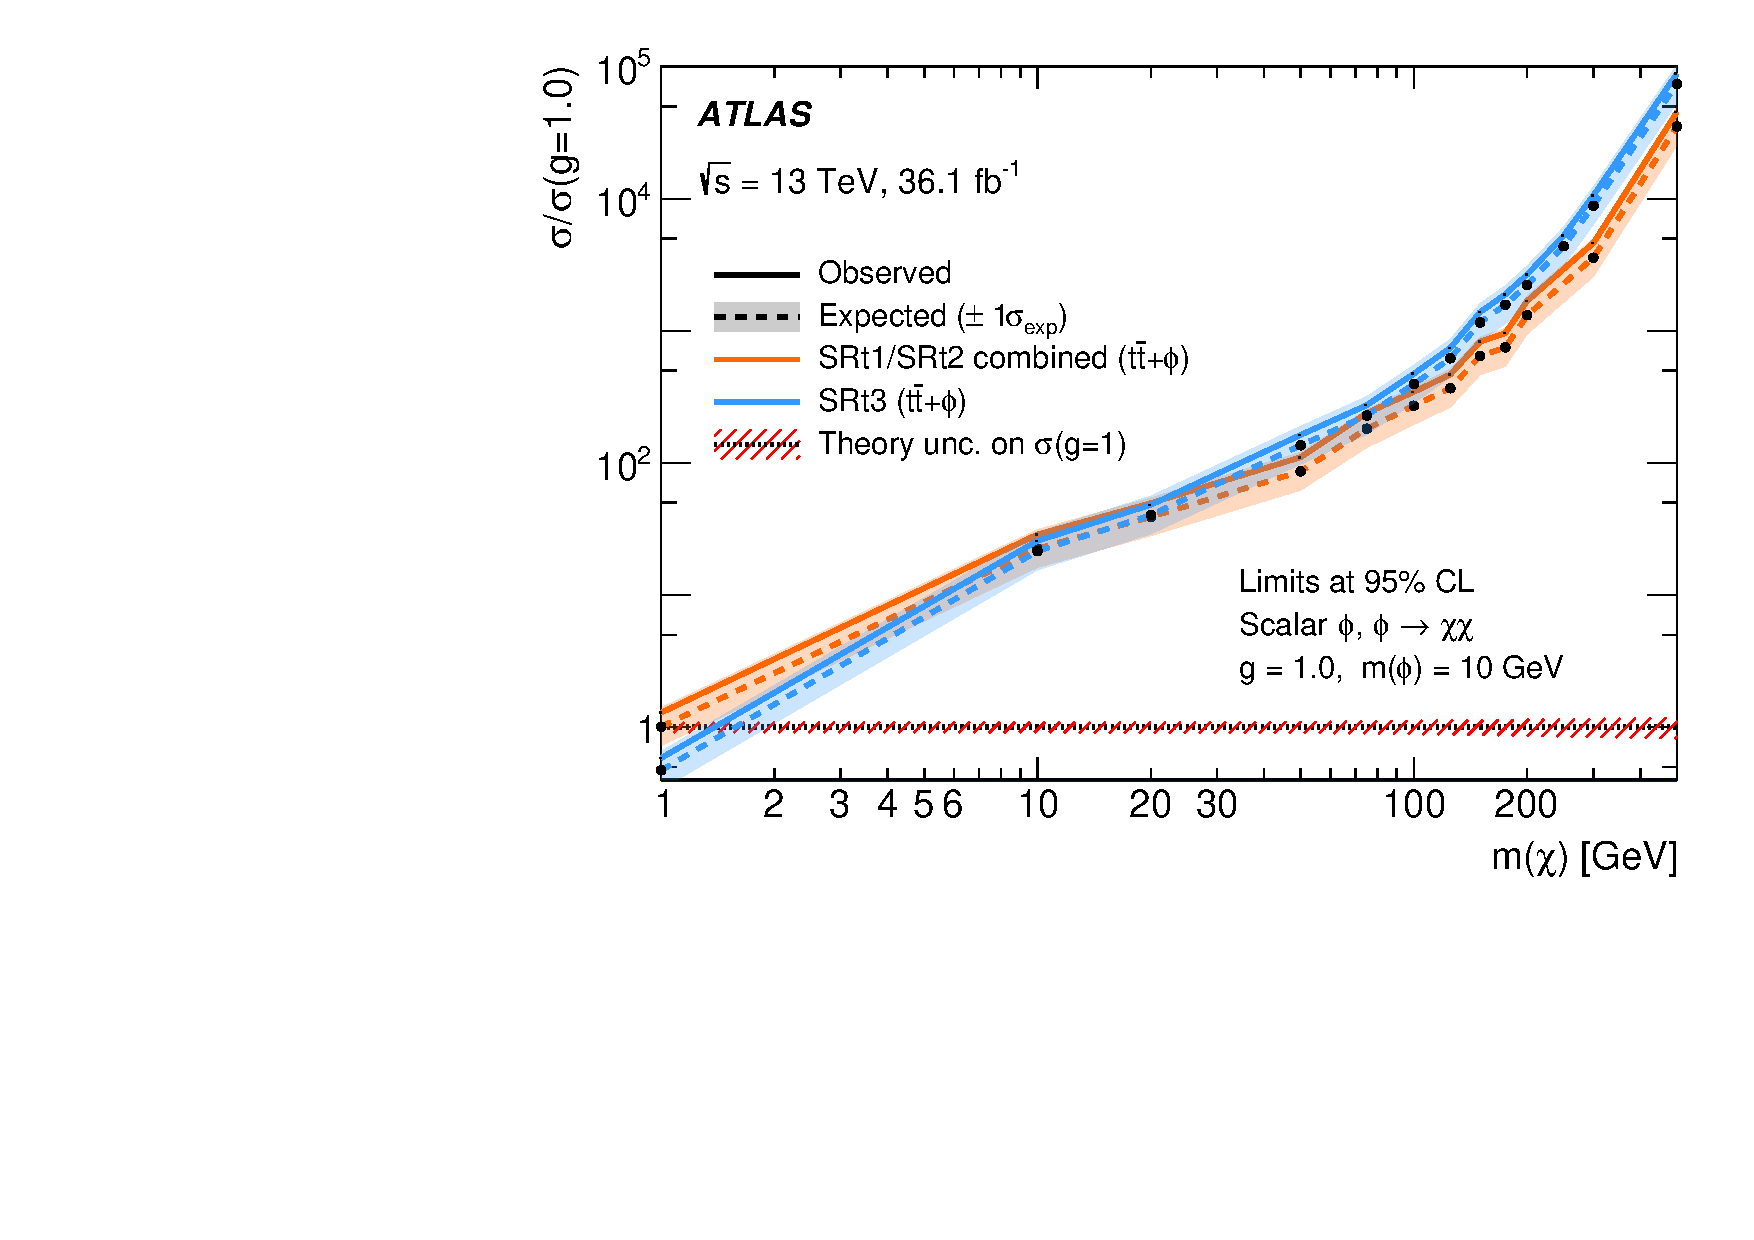
\includegraphics[width=.9\textwidth]{appA/final_scalar_SR1_offshell}}
			\subbottom[]{
				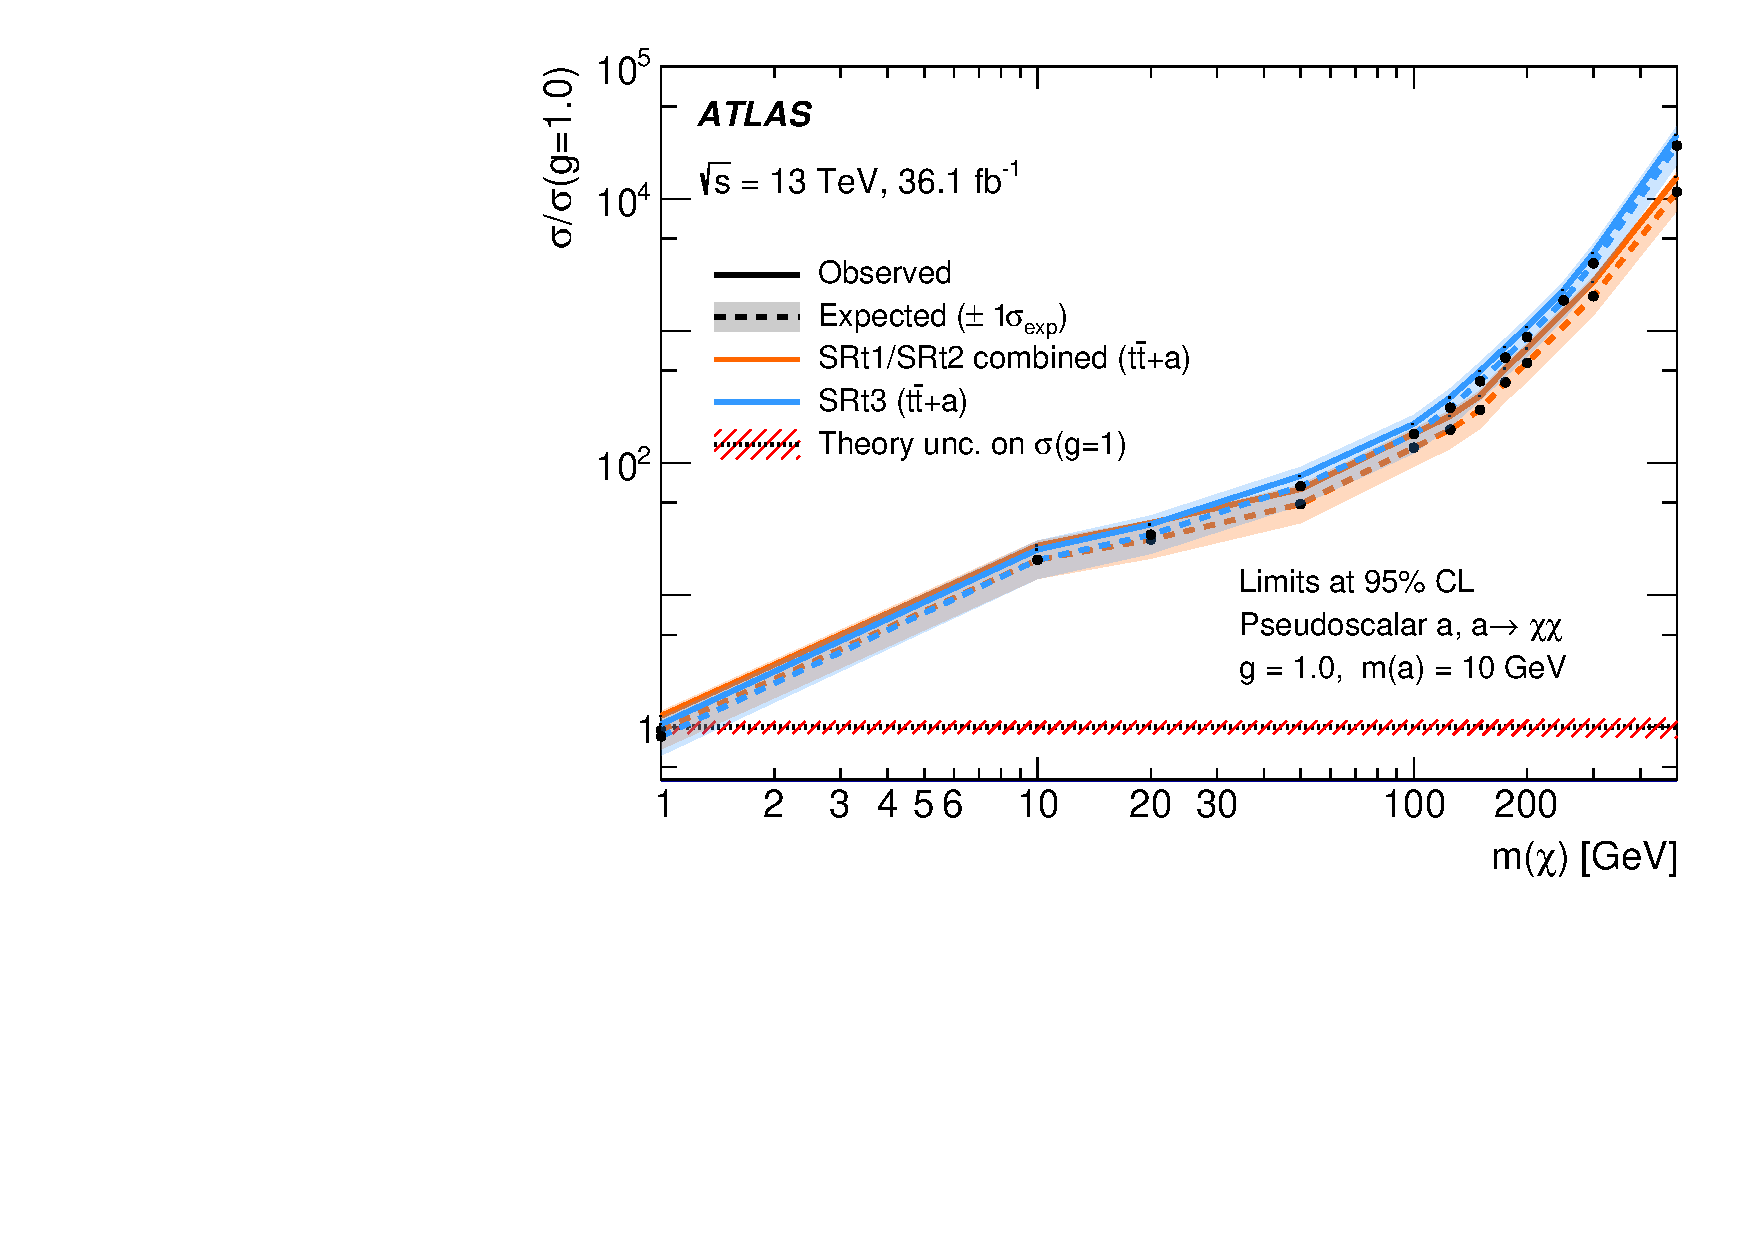
\includegraphics[width=.9\textwidth]{appA/final_pseudo_SR1_offshell}}
			\caption{Exclusion limits for colour-neutral $\ttbar+\phi$ scalar (a) and $\ttbar+a$ pseudoscalar (b)  models as a function of the DM mass for a mediator mass of $10\;\GeV$. The limits are calculated at 95\% CL and are expressed in terms of the ratio of the excluded cross-section to the nominal cross-section for a coupling assumption of $g = g_q = g_\chi = 1$, where $g_\chi$ is the DM–mediator coupling, and $g_q$ the flavour-universal SM–mediator coupling. The solid (dashed) lines shows the observed (expected) exclusion limits for the different signal regions, according to the colour code specified in the legend. To derive the results for the fully hadronic \ttbar\ final state the region SRt1 or SRt2 providing the better expected sensitivity is used (taken from~\cite{DMhf}.}
			\label{fig:dmresultschi}
		\end{figure}